\documentclass[a4paper,11pt]{article}

\usepackage[left=25mm,right=25mm,top=25mm,bottom=25mm]{geometry}
\usepackage[T1]{fontenc}
\usepackage{xcolor}
\usepackage[most]{tcolorbox}
\usepackage{listings}
\usepackage[hidelinks,colorlinks=true,linkcolor=conceptpurple,urlcolor=keywordblue]{hyperref}
\usepackage{parskip}
\usepackage{booktabs}
\usepackage{amsmath,amssymb}
\usepackage{graphicx}
\usepackage{enumitem}
\usepackage{fancyhdr}
\usepackage{titlesec}
\usepackage{tikz}
\usetikzlibrary{arrows.meta,positioning,shapes.geometric,calc}
\tcbuselibrary{breakable}

\definecolor{codebg}{RGB}{245,245,248}
\definecolor{conceptpurple}{RGB}{100,40,150}
\definecolor{keywordblue}{RGB}{0,0,180}
\definecolor{stringred}{RGB}{160,0,0}
\definecolor{commentgreen}{RGB}{0,120,0}
\definecolor{warningyellow}{RGB}{255,200,0}
\definecolor{warningbg}{RGB}{255,250,230}
\definecolor{successgreen}{RGB}{0,140,0}
\definecolor{successbg}{RGB}{230,255,235}
\definecolor{analogybg}{RGB}{235,245,255}
\definecolor{analogyblue}{RGB}{0,80,160}
\definecolor{philosophybg}{RGB}{245,235,255}
\definecolor{deepdivebg}{RGB}{240,248,240}

\lstset{
  basicstyle=\ttfamily\small,
  backgroundcolor=\color{codebg},
  frame=single,
  numbers=left,
  numberstyle=\tiny\color{gray},
  keywordstyle=\color{keywordblue}\bfseries,
  stringstyle=\color{stringred},
  commentstyle=\color{commentgreen}\itshape,
  breaklines=true,
  breakatwhitespace=true,
  showstringspaces=false,
  tabsize=2,
  captionpos=b,
}

\newtcolorbox{analogybox}[1][]{
  colback=analogybg, colframe=analogyblue,
  fonttitle=\bfseries, title={Analogy: #1},
  breakable, arc=4pt
}

\newtcolorbox{conceptbox}[1][]{
  colback=white, colframe=conceptpurple,
  fonttitle=\bfseries\color{white}, coltitle=white,
  colbacktitle=conceptpurple,
  title={Key Concept: #1}, breakable, arc=4pt
}

\newtcolorbox{warningbox}[1][]{
  colback=warningbg, colframe=orange,
  fonttitle=\bfseries, title={\textbf{!}~Watch Out: #1},
  breakable, arc=4pt
}

\newtcolorbox{expertbox}[1][]{
  colback=deepdivebg, colframe=successgreen,
  fonttitle=\bfseries, title={Expert Insight: #1},
  breakable, arc=4pt
}

\newtcolorbox{philosophybox}[1][]{
  colback=philosophybg, colframe=conceptpurple!60,
  fonttitle=\bfseries\itshape, title={Bigger Picture: #1},
  breakable, arc=4pt
}

\newtcolorbox{revealbox}[1][]{
  colback=codebg, colframe=stringred,
  fonttitle=\bfseries, title={What You'll Realize Later: #1},
  breakable, arc=4pt
}

\title{\textbf{Demystifying GPU Performance Mechanisms}\\[0.4em]
  \large A First-Principles Guide to Warp Divergence, Coalesced Memory Access, and Pointer Indirection}
\author{Antigravity Systems Engineering Group}
\date{\today}

\begin{document}
\maketitle

\begin{abstract}
High-throughput parallel processors---such as modern Graphics Processing Units (GPUs)---are capable of executing tens of thousands of concurrent operations per microsecond. However, programmers arriving from CPU architectures frequently encounter catastrophic performance bottlenecks when their code runs on GPU hardware. A shader that appears theoretically parallel in high-level code can easily suffer a $10\times$ to $50\times$ slowdown due to subtle hardware-level mismatches.

This document teaches the three fundamental hardware mechanisms that govern GPU compute performance: \textbf{Warp Divergence} (how lockstep execution penalizes branchy code), \textbf{Coalesced Memory Access} (how the hardware memory bus bundles simultaneous memory reads into unified cache lines), and \textbf{Zero Pointer Indirection} (why arithmetic indexing outclasses pointer-based heap chasing). 

By building intuition from the physical silicon level up to high-level compute shaders (such as WGSL and CUDA), this guide equips software engineers to understand \textit{why} algorithmic trade-offs are made in systems like high-performance fuzzy search engines and database engines.
\end{abstract}

\tableofcontents
\newpage

%% =========================================================================
\section{The Core Mental Model: CPU vs. GPU Silicon}
%% =========================================================================

To understand why GPUs care so intensely about memory layout and branch predictability, we must first examine the physical priorities that dictated their silicon designs.

\begin{figure}[htbp]
\centering
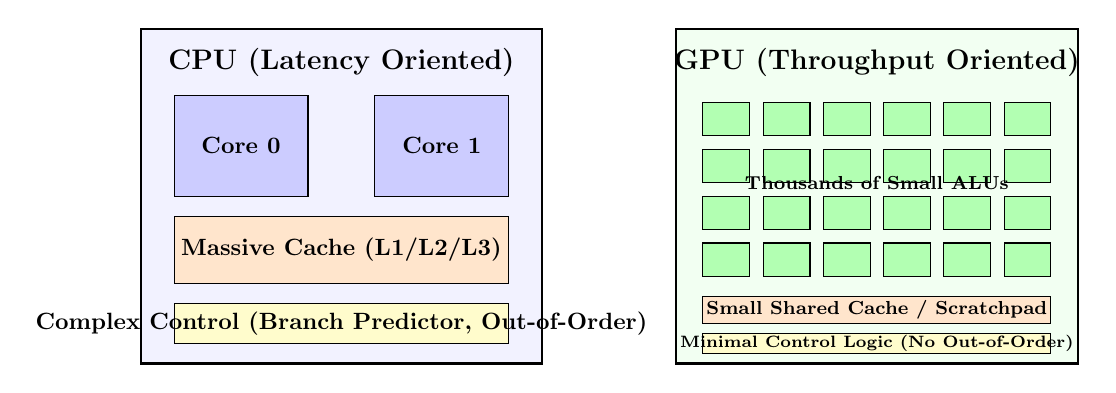
\begin{tikzpicture}[scale=0.85, every node/.style={transform shape}]
  % CPU Box
  \draw[thick, fill=blue!5] (0,0) rectangle (6,5);
  \node[font=\bfseries\large] at (3,4.5) {CPU (Latency Oriented)};
  
  \draw[fill=blue!20] (0.5,2.5) rectangle (2.5,4);
  \node at (1.5,3.25) {\textbf{Core 0}};
  \draw[fill=blue!20] (3.5,2.5) rectangle (5.5,4);
  \node at (4.5,3.25) {\textbf{Core 1}};
  
  \draw[fill=orange!20] (0.5,1.2) rectangle (5.5,2.2);
  \node at (3,1.7) {\textbf{Massive Cache (L1/L2/L3)}};
  
  \draw[fill=yellow!20] (0.5,0.3) rectangle (5.5,0.9);
  \node at (3,0.6) {\textbf{Complex Control (Branch Predictor, Out-of-Order)}};

  % GPU Box
  \draw[thick, fill=green!5] (8,0) rectangle (14,5);
  \node[font=\bfseries\large] at (11,4.5) {GPU (Throughput Oriented)};
  
  % Grid of tiny ALUs
  \foreach \x in {0,1,2,3,4,5} {
    \foreach \y in {0,1,2,3} {
      \draw[fill=green!30] (8.4 + \x*0.9, 1.3 + \y*0.7) rectangle (9.1 + \x*0.9, 1.8 + \y*0.7);
    }
  }
  \node[font=\footnotesize] at (11,2.7) {\textbf{Thousands of Small ALUs}};
  
  \draw[fill=orange!20] (8.4,0.6) rectangle (13.6,1.0);
  \node[font=\footnotesize] at (11,0.8) {\textbf{Small Shared Cache / Scratchpad}};
  
  \draw[fill=yellow!20] (8.4,0.15) rectangle (13.6,0.45);
  \node[font=\scriptsize] at (11,0.3) {\textbf{Minimal Control Logic (No Out-of-Order)}};
\end{tikzpicture}
\caption{Architectural comparison: CPU cores devote silicon to giant caches and speculative execution units to minimize latency for a single thread. GPUs devote silicon almost entirely to raw Arithmetic Logic Units (ALUs) to maximize aggregate throughput.}
\label{fig:cpu_vs_gpu}
\end{figure}

\subsection{Latency Optimization vs. Throughput Optimization}

A Central Processing Unit (CPU) is built like a \textbf{Formula 1 racing car}. Its sole objective is to complete an intricate, unpredictable sequence of tasks as fast as physically possible. To achieve this:
\begin{itemize}[leftmargin=1.5em]
  \item It features sophisticated \textbf{branch predictors} that guess which way an \texttt{if/else} branch will go hundreds of instructions in advance.
  \item It features \textbf{Out-of-Order (OoO) execution engines} that dynamically re-order independent machine instructions to keep the pipeline full.
  \item It dedicates more than $60\%$ of its physical chip area to multi-level SRAM caches (\textbf{L1, L2, and L3 caches}) so data is rarely fetched from high-latency main RAM.
\end{itemize}

A Graphics Processing Unit (GPU) is built like a \textbf{freight train}. It does not move any individual grain of sand faster than a race car, but it carries thousands of tons simultaneously. To pack thousands of arithmetic execution units onto a single silicon die:
\begin{itemize}[leftmargin=1.5em]
  \item \textbf{No complex branch predictors:} The hardware cannot afford space for dynamic speculative engines per core.
  \item \textbf{No Out-of-Order logic:} Instructions are executed strictly in order.
  \item \textbf{Tiny caches per thread:} Rather than hiding memory latency with giant per-core caches, the GPU hides latency by \textbf{context switching between thousands of active threads} instantly. If Thread Group A is waiting for data from VRAM, the hardware scheduler pauses Group A and immediately instructs the ALUs to compute calculations for Group B.
\end{itemize}

\begin{conceptbox}[The Core GPU Rule]
On a CPU, performance is achieved by making an individual thread's path as short and uninterrupted as possible. On a GPU, performance is achieved by ensuring that \textbf{thousands of threads do exactly the same thing at the exact same time}.
\end{conceptbox}

\newpage

%% =========================================================================
\section{Mechanism 1: Warp Divergence (SIMT Execution)}
%% =========================================================================

\subsection{Motivation: Why Don't GPUs Have Independent Cores?}

If a modern GPU has 4,096 ALUs, one might assume there are 4,096 independent microprocessors each reading their own instruction stream. If this were true, the silicon required to fetch, decode, and schedule instructions would consume the entire chip, leaving no room for actual arithmetic units.

To solve this, hardware designers invented \textbf{SIMD} (\textit{Single Instruction, Multiple Data}) and its GPU evolution, \textbf{SIMT} (\textit{Single Instruction, Multiple Threads}). 

Instead of giving each execution unit its own instruction decoder, the GPU groups threads into lockstep clusters called:
\begin{itemize}
  \item \textbf{Warps} on NVIDIA GPUs (32 threads).
  \item \textbf{Wavefronts} on AMD GPUs (usually 32 or 64 threads) and Intel / Apple Silicon execution units.
\end{itemize}

A single instruction fetch unit broadcasts \textbf{one instruction} to all 32 threads in the warp simultaneously.

\begin{analogybox}[The Marching Band]
Imagine a military marching band of 32 musicians marching in a synchronized line. The drill sergeant (the instruction dispatcher) barks a single command: \textit{"Step forward with your left foot!"} All 32 musicians take the exact same step at the exact same instant. 

Now imagine the sergeant commands: \textit{"If your shoe size is odd, jump to the left; if your shoe size is even, jump to the right!"}

Because the musicians cannot physically move in opposite directions simultaneously while maintaining their formation, the band must \textbf{serialize}:
\begin{enumerate}
  \item The musicians with even shoe sizes freeze and stand completely motionless while the odd-sized musicians jump left.
  \item Then, the odd-sized musicians freeze while the even-sized musicians jump right.
\end{enumerate}
Although each musician only executed one jump, the entire band took \textbf{twice as long} to finish the exercise, and half the band was completely idle during each step.
\end{analogybox}

\subsection{The Mechanics of Warp Divergence}

When threads within the same warp take different branches of a conditional statement (\texttt{if/else}, \texttt{switch}, or loops with variable iteration counts), the warp undergoes \textbf{Warp Divergence}.

\begin{figure}[htbp]
\centering
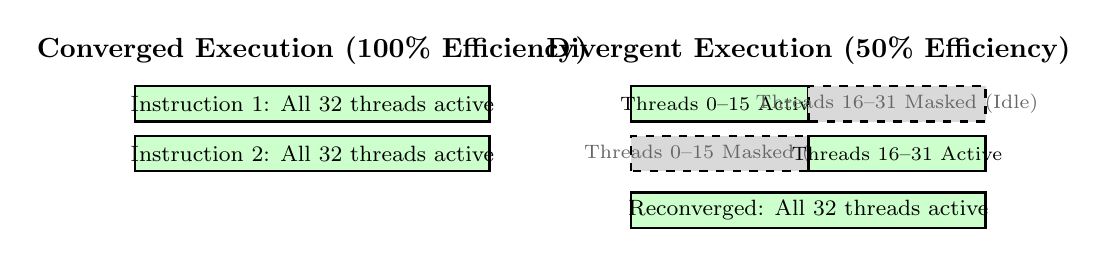
\begin{tikzpicture}[scale=0.9]
  % Uniform Execution
  \node[font=\bfseries] at (2.5, 3.5) {Converged Execution (100\% Efficiency)};
  \draw[fill=green!20, thick] (0, 2.5) rectangle (5, 3.0);
  \node[font=\footnotesize] at (2.5, 2.75) {Instruction 1: All 32 threads active};
  \draw[fill=green!20, thick] (0, 1.8) rectangle (5, 2.3);
  \node[font=\footnotesize] at (2.5, 2.05) {Instruction 2: All 32 threads active};

  % Divergent Execution
  \node[font=\bfseries] at (9.5, 3.5) {Divergent Execution (50\% Efficiency)};
  % Branch A
  \draw[fill=green!20, thick] (7, 2.5) rectangle (9.5, 3.0);
  \node[font=\scriptsize] at (8.25, 2.75) {Threads 0--15 Active};
  \draw[fill=gray!30, dashed, thick] (9.5, 2.5) rectangle (12, 3.0);
  \node[font=\scriptsize, color=gray!80!black] at (10.75, 2.75) {Threads 16--31 Masked (Idle)};
  
  % Branch B
  \draw[fill=gray!30, dashed, thick] (7, 1.8) rectangle (9.5, 2.3);
  \node[font=\scriptsize, color=gray!80!black] at (8.25, 2.05) {Threads 0--15 Masked (Idle)};
  \draw[fill=green!20, thick] (9.5, 1.8) rectangle (12, 2.3);
  \node[font=\scriptsize] at (10.75, 2.05) {Threads 16--31 Active};

  % Reconverge
  \draw[fill=green!20, thick] (7, 1.0) rectangle (12, 1.5);
  \node[font=\footnotesize] at (9.5, 1.25) {Reconverged: All 32 threads active};
\end{tikzpicture}
\caption{Warp Divergence in hardware. The execution mask disables inactive threads while the instruction pipeline steps through divergent execution paths sequentially.}
\label{fig:warp_divergence}
\end{figure}

The GPU hardware handles divergence through \textbf{Execution Masking}:
\begin{enumerate}
  \item The warp encounters a branch: \texttt{if (condition) \{ Path A \} else \{ Path B \}}.
  \item The hardware computes a 32-bit bitmask where bit $k = 1$ if thread $k$ evaluated \texttt{condition == true}.
  \item The instruction unit executes \textbf{Path A}. Threads with a $0$ bit are physically disabled (masked out); their ALUs burn clock cycles doing nothing, and any register writes are inhibited.
  \item The hardware flips the bitmask and executes \textbf{Path B}. Threads with a $1$ bit are disabled.
  \item The threads \textbf{reconverge} after the conditional block, restoring $100\%$ ALU utilization.
\end{enumerate}

\subsection{Mathematical Formalism of Divergence Penalty}

Let a warp have $W$ threads ($W = 32$). Suppose a conditional block contains $M$ divergent branches $B_1, B_2, \dots, B_M$, where each branch $B_j$ requires $T(B_j)$ clock cycles to execute.

If all threads take the same branch $B_k$, the total time is simply:
\begin{equation}
  T_{\text{converged}} = T(B_k)
\end{equation}

If the threads diverge across all $M$ branches, the execution is serialized:
\begin{equation}
  T_{\text{divergent}} = \sum_{j=1}^{M} T(B_j)
\end{equation}

The average computational efficiency $\eta_{\text{ALU}}$ of the warp is given by:
\begin{equation}
  \eta_{\text{ALU}} = \frac{\sum_{j=1}^{M} n_j \cdot T(B_j)}{W \cdot \sum_{j=1}^{M} T(B_j)}
\end{equation}
where $n_j$ is the number of active threads taking branch $B_j$ (such that $\sum n_j \le W$). If a single thread takes a branch with 100 instructions while the other 31 threads take a branch with 1 instruction, 31 ALUs sit idle for 100 cycles.

\subsection{Application: Why Fixed String Bounds ($N \le 59$) Were Chosen}

In string searching (fuzzy or substring matching), comparison loops depend on string length:
\begin{lstlisting}[language=C]
for (var i = 0u; i < str_len; i++) { ... }
\end{lstlisting}

If Thread 0 is evaluating a string of length 5, and Thread 1 in the same warp is evaluating a string of length 300:
\begin{itemize}
  \item Thread 0 completes its 5 iterations in nanoseconds.
  \item Because Thread 1 must execute 300 iterations, the entire warp is forced to execute 300 iterations.
  \item Thread 0 sits masked out and idle for 295 iterations ($98.3\%$ wasted ALU time).
\end{itemize}

By clamping strings to a fixed 64-byte slot with a strict upper bound of $\min(\text{str\_len}, 59)$, \textbf{no thread in any warp can ever execute more than 59 iterations}. This established a hard ceiling on warp divergence, ensuring predictable, high-speed execution across diverse datasets.

\newpage

%% =========================================================================
\section{Mechanism 2: Coalesced Memory Access \& Cache Line Alignment}
%% =========================================================================

\subsection{Motivation: The Memory Bus Bottleneck}

Silicon ALUs can perform floating-point and integer math in a fraction of a nanosecond. However, fetching data across the physical traces of a circuit board from external Video RAM (VRAM / GDDR6 / LPDDR5) takes anywhere from \textbf{200 to 500 clock cycles}.

If every thread in a 32-thread warp independently requested an isolated, random 4-byte integer from memory, the GPU's memory controller would have to perform \textbf{32 separate memory bus transactions}. The ALUs would stall for thousands of cycles waiting for the memory bus to service these requests one by one.

\subsection{The Physics of Coalescing}

To prevent memory bus saturation, modern GPUs feature a hardware unit called the \textbf{Memory Coalescer}. 

VRAM is physically organized into fixed-size cache chunks known as \textbf{Cache Lines} (typically 64 bytes or 128 bytes wide). A GPU cannot read a single isolated byte from VRAM; it can only read an entire 64-byte or 128-byte cache block in a single burst transaction.

\begin{figure}[htbp]
\centering
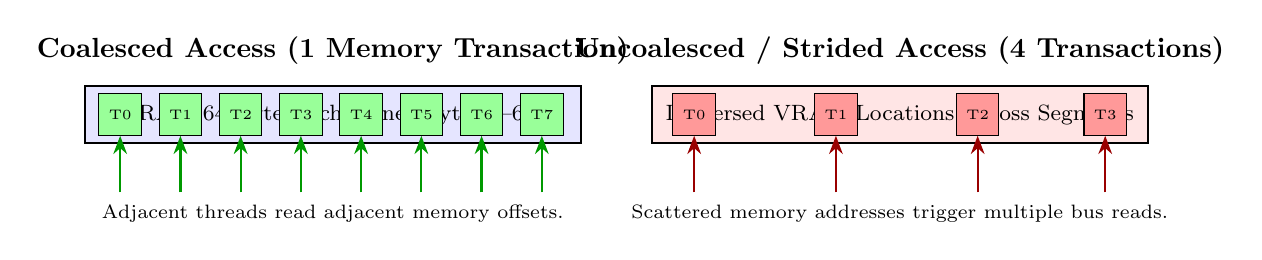
\begin{tikzpicture}[scale=0.9]
  % Coalesced Access
  \node[font=\bfseries] at (3.5, 3.5) {Coalesced Access (1 Memory Transaction)};
  \draw[thick, fill=blue!10] (0, 2.2) rectangle (7, 3.0);
  \node[font=\footnotesize] at (3.5, 2.6) {VRAM 64-Byte Cache Line (Bytes 0--63)};
  
  \foreach \i in {0,1,2,3,4,5,6,7} {
    \draw[fill=green!40] (0.2 + \i*0.85, 2.3) rectangle (0.8 + \i*0.85, 2.9);
    \node[font=\tiny] at (0.5 + \i*0.85, 2.6) {T\i};
    \draw[-{Stealth}, thick, green!60!black] (0.5 + \i*0.85, 1.5) -- (0.5 + \i*0.85, 2.3);
  }
  \node[font=\scriptsize] at (3.5, 1.2) {Adjacent threads read adjacent memory offsets.};

  % Uncoalesced Access
  \node[font=\bfseries] at (11.5, 3.5) {Uncoalesced / Strided Access (4 Transactions)};
  \draw[thick, fill=red!10] (8, 2.2) rectangle (15, 3.0);
  \node[font=\footnotesize] at (11.5, 2.6) {Dispersed VRAM Locations Across Segments};
  
  \draw[fill=red!40] (8.3, 2.3) rectangle (8.9, 2.9);
  \node[font=\tiny] at (8.6, 2.6) {T0};
  \draw[-{Stealth}, thick, red!60!black] (8.6, 1.5) -- (8.6, 2.3);

  \draw[fill=red!40] (10.3, 2.3) rectangle (10.9, 2.9);
  \node[font=\tiny] at (10.6, 2.6) {T1};
  \draw[-{Stealth}, thick, red!60!black] (10.6, 1.5) -- (10.6, 2.3);

  \draw[fill=red!40] (12.3, 2.3) rectangle (12.9, 2.9);
  \node[font=\tiny] at (12.6, 2.6) {T2};
  \draw[-{Stealth}, thick, red!60!black] (12.6, 1.5) -- (12.6, 2.3);

  \draw[fill=red!40] (14.1, 2.3) rectangle (14.7, 2.9);
  \node[font=\tiny] at (14.4, 2.6) {T3};
  \draw[-{Stealth}, thick, red!60!black] (14.4, 1.5) -- (14.4, 2.3);

  \node[font=\scriptsize] at (11.5, 1.2) {Scattered memory addresses trigger multiple bus reads.};
\end{tikzpicture}
\caption{Coalesced versus uncoalesced memory access. When threads access consecutive, aligned memory, the hardware coalesces all reads into a single physical bus transaction.}
\label{fig:coalescing}
\end{figure}

\begin{analogybox}[The Mail Delivery Truck]
Suppose a delivery truck carries mail to a suburban neighborhood. 
\begin{itemize}
  \item \textbf{Coalesced Access:} The truck parks in front of a row of 32 adjacent houses. The mail carrier steps out, drops one letter into each box along the block in a single stop, and drives away. Total delivery time: 1 minute.
  \item \textbf{Uncoalesced Access:} 32 people in different corners of a metropolitan area each order a package. The truck must drive to 32 completely different neighborhoods, parking 32 separate times. Total delivery time: 3 hours.
\end{itemize}
The total payload delivered (32 letters) is identical, but the transport overhead is orders of magnitude worse.
\end{analogybox}

\subsection{Why 64 Bytes per Slot?}

In high-performance GPU programming, data layouts are engineered to align with hardware cache line boundaries:
\begin{enumerate}
  \item \textbf{Exact Power-of-Two Alignment ($2^6 = 64$):} 64 bytes is the fundamental L1 cache line size on major modern GPU architectures.
  \item \textbf{Coalesced Row Headers:} When 16 consecutive threads in a workgroup fetch the length header of their respective strings:
  \begin{equation}
    \text{Address}(k) = k \times 64 \quad (k \in [0, 15])
  \end{equation}
  The memory controller detects that the base addresses are aligned to 64-byte boundaries. When consecutive threads read word 0 of their slot, the memory requests can be mapped across memory channels with zero split-transaction penalties.
\end{enumerate}

\begin{expertbox}[The Effective Bandwidth Equation]
Memory efficiency is measured by the ratio of useful bytes received to total bytes transferred:
\begin{equation}
  \text{Bus Utilization} = \frac{\text{Requested Bytes}}{\text{Transactions} \times \text{Cache Line Size}}
\end{equation}
If 32 threads request 4 bytes each (128 bytes total), and their addresses fall into 32 separate 64-byte cache lines, the bus transfers $32 \times 64 = 2,048$ bytes. The bus utilization is $\frac{128}{2048} \approx 6.25\%$, wasting $93.75\%$ of the memory bandwidth!
\end{expertbox}

\newpage

%% =========================================================================
\section{Mechanism 3: Zero Pointer Indirection}
%% =========================================================================

\subsection{The CPU Tradition: Pointer-Based Data Structures}

In traditional CPU software engineering (Java, Python, C++, TypeScript), data structures are built from pointers and references:
\begin{itemize}
  \item An array of strings is an array of \textbf{pointers} (memory addresses) pointing to disjoint objects scattered across the heap: \texttt{char* items[]}.
  \item Trees, linked lists, and hash maps rely on nodes holding pointers to other nodes.
\end{itemize}

On a CPU, this is often acceptable because large caches and hardware prefetchers notice when you traverse memory. On a GPU, pointer chasing is one of the most destructive architectural patterns possible.

\subsection{The Cost of Pointer Chasing on GPUs}

Consider what happens when a GPU thread wants to read a string via an indirect pointer:

\begin{figure}[htbp]
\centering
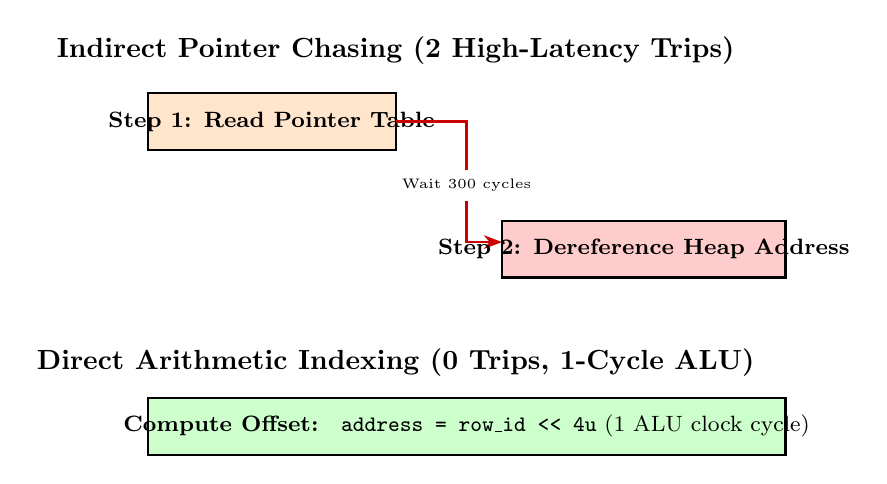
\begin{tikzpicture}[scale=0.9]
  % Indirect access
  \node[font=\bfseries] at (3.5, 4.2) {Indirect Pointer Chasing (2 High-Latency Trips)};
  
  \draw[fill=orange!20, thick] (0, 2.8) rectangle (3.5, 3.6);
  \node[font=\footnotesize] at (1.75, 3.2) {\textbf{Step 1: Read Pointer Table}};
  
  \draw[-{Stealth}, thick, red!80!black] (3.5, 3.2) -- (4.5, 3.2) -- (4.5, 1.5) -- (5.0, 1.5);
  \node[font=\tiny, fill=white] at (4.5, 2.3) {Wait 300 cycles};

  \draw[fill=red!20, thick] (5.0, 1.0) rectangle (9.0, 1.8);
  \node[font=\footnotesize] at (7.0, 1.4) {\textbf{Step 2: Dereference Heap Address}};

  % Direct Arithmetic
  \node[font=\bfseries] at (3.5, -0.2) {Direct Arithmetic Indexing (0 Trips, 1-Cycle ALU)};
  \draw[fill=green!20, thick] (0, -1.5) rectangle (9.0, -0.7);
  \node[font=\footnotesize] at (4.5, -1.1) {\textbf{Compute Offset: } \texttt{address = row\_id << 4u} (1 ALU clock cycle)};
\end{tikzpicture}
\caption{Pointer chasing versus direct arithmetic addressing. Pointer dereferencing forces the thread to stall on two dependent memory roundtrips before it can examine a single character.}
\label{fig:pointer_indirection}
\end{figure}

\begin{enumerate}
  \item \textbf{Trip 1 (Read Pointer):} The thread reads the pointer table at \texttt{table[row\_id]} to discover where the string lives in memory. The thread stalls for 200--400 cycles waiting for the memory controller.
  \item \textbf{Trip 2 (Dereference):} The pointer arrives. The thread can now issue a \textit{second} memory read to the heap address it just learned. The thread stalls for another 200--400 cycles.
  \item \textbf{Uncoalesced Chaos:} Because memory allocators place strings in arbitrary heap locations, adjacent threads in the warp now possess completely unrelated memory addresses. The memory controller is forced to break the warp's read into dozens of serialized, uncoalesced bus requests.
\end{enumerate}

\subsection{The Solution: Arithmetic Slot Addressing}

In our 64-byte slot design, \textbf{there are no pointers}. The memory location of any record is computed purely through integer arithmetic:

\begin{equation}
  \text{Byte Address}(\text{row\_id}) = \text{row\_id} \times 64 = \text{row\_id} \ll 6
\end{equation}

In terms of 32-bit words (\texttt{u32}, 4 bytes each):
\begin{equation}
  \text{Word Index}(\text{row\_id}) = \text{row\_id} \times 16 = \text{row\_id} \ll 4
\end{equation}

\begin{lstlisting}[language=C]
// Zero pointers. Zero memory lookups to find the string.
// A 1-cycle bit-shift directly gives the record's location:
fn get_char(row_id: u32, pos: u32) -> u32 {
    let word_idx = 1u + (pos >> 2u);
    let shift = (pos & 3u) * 8u;
    return (records[row_id * 16u + word_idx] >> shift) & 0xFFu;
}
\end{lstlisting}

\begin{conceptbox}[Why Bit-Shifting is Free]
Multiplying by 16 is equivalent to a logical bit-shift left by 4 bits (\texttt{x << 4u}). Modern GPU ALUs execute bit-shifts in a single clock cycle ($< 0.5$ nanoseconds). Replacing a 300-cycle memory read with a 1-cycle bit-shift represents an instantaneous $\mathbf{300\times}$ latency reduction for addressing calculations.
\end{conceptbox}

\newpage

%% =========================================================================
\section{Engineering Tradeoffs: Fixed Slots vs. Dynamic Heaps}
%% =========================================================================

In the previous version of our search engine, we enforced a strict 64-byte slot ($59$ character maximum). In this release, we removed that limit to support real-world, arbitrarily long paths. 

Understanding the engineering trade-offs between these two models is essential for systems design.

\begin{table}[htbp]
\centering
\small
\begin{tabular}{@{}lll@{}}
\toprule
\textbf{Metric / Concern} & \textbf{Fixed 64-Byte Slot Model} & \textbf{Dynamic Offset Table Model} \\
\midrule
\textbf{Addressing Overhead} & Zero (Pure bit-shift: \texttt{row\_id << 4u}) & 1 Memory Read (\texttt{offsets[row\_id]}) \\
\textbf{Memory Allocation} & Fixed: $N \times 64$ bytes & Exact: $\sum \text{len}_i + (N+1) \times 4$ bytes \\
\textbf{VRAM Waste on Short Strings} & High (10-char string wastes 50 bytes) & Zero (Zero padding characters) \\
\textbf{Maximum String Length} & Strictly capped at 59 characters & Unlimited (100, 500, or 2,000+ chars) \\
\textbf{Warp Divergence Risk} & Bounded (Never exceeds 59 iterations) & Unbounded if string lengths vary widely \\
\textbf{PCIe Upload Size} & Larger (Uploads padding zeroes) & Minimal (Uploads only real characters) \\
\textbf{Real-World Viability} & Benchmark only (truncates paths) & Production-ready for arbitrary datasets \\
\bottomrule
\end{tabular}
\caption{Comparison of memory storage strategies on GPU hardware.}
\label{tab:tradeoffs}
\end{table}

\subsection{Why the Apache Arrow / Offset Array Model is the Industry Standard}

To remove the 59-character limit without regressing to scattered heap pointers, we implemented the \textbf{Offsets Buffer Architecture} (pioneered by Apache Arrow and DuckDB):

\begin{figure}[htbp]
\centering
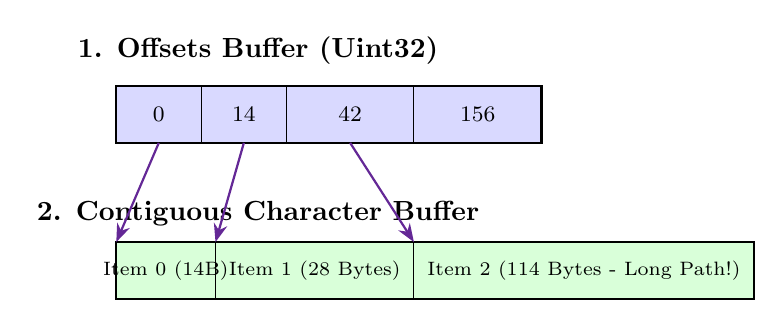
\begin{tikzpicture}[scale=0.9]
  % Offsets Buffer
  \node[font=\bfseries] at (2.0, 2.5) {1. Offsets Buffer (Uint32)};
  \draw[fill=blue!15, thick] (0, 1.2) rectangle (6, 2.0);
  \node[font=\footnotesize] at (0.6, 1.6) {0};
  \draw (1.2, 1.2) -- (1.2, 2.0);
  \node[font=\footnotesize] at (1.8, 1.6) {14};
  \draw (2.4, 1.2) -- (2.4, 2.0);
  \node[font=\footnotesize] at (3.3, 1.6) {42};
  \draw (4.2, 1.2) -- (4.2, 2.0);
  \node[font=\footnotesize] at (5.1, 1.6) {156};

  % Records Buffer
  \node[font=\bfseries] at (2.0, 0.2) {2. Contiguous Character Buffer};
  \draw[fill=green!15, thick] (0, -1.0) rectangle (9, -0.2);
  \node[font=\scriptsize] at (0.7, -0.6) {Item 0 (14B)};
  \draw (1.4, -1.0) -- (1.4, -0.2);
  \node[font=\scriptsize] at (2.8, -0.6) {Item 1 (28 Bytes)};
  \draw (4.2, -1.0) -- (4.2, -0.2);
  \node[font=\scriptsize] at (6.6, -0.6) {Item 2 (114 Bytes - Long Path!)};

  % Pointers
  \draw[-{Stealth}, thick, conceptpurple] (0.6, 1.2) -- (0.0, -0.2);
  \draw[-{Stealth}, thick, conceptpurple] (1.8, 1.2) -- (1.4, -0.2);
  \draw[-{Stealth}, thick, conceptpurple] (3.3, 1.2) -- (4.2, -0.2);
\end{tikzpicture}
\caption{The Arrow-style offset table model: All characters are packed sequentially into a single contiguous buffer with zero gap padding. Row $k$ starts at byte \texttt{offsets[k]} and has length \texttt{offsets[k+1] - offsets[k]}.}
\label{fig:arrow_layout}
\end{figure}

This architecture strikes the ideal engineering balance:
\begin{enumerate}
  \item \textbf{No Scattered Heap Dereferencing:} Both the \texttt{offsets} buffer and the \texttt{records} buffer are contiguous arrays stored in VRAM.
  \item \textbf{Coalesced Offset Reads:} When threads 0 to 31 in a warp request their string boundaries:
  \begin{equation}
    \text{start} = \text{offsets}[\text{row\_id}], \quad \text{end} = \text{offsets}[\text{row\_id} + 1]
  \end{equation}
  The 32 threads read 32 adjacent 4-byte integers. The memory coalescer satisfies all 32 thread requests in a \textbf{single 128-byte cache read}!
  \item \textbf{Zero Truncation:} Whether a path is 12 characters or 350 characters, it is stored completely and accurately.
\end{enumerate}

\newpage

%% =========================================================================
\section{Viva, Interview, and Systems Mastery Questions}
%% =========================================================================

\begin{enumerate}[leftmargin=2.0em, label=\textbf{Q\arabic*:}]
  \item \textbf{Why does a GPU warp execute both sides of an \texttt{if/else} branch if at least one thread evaluates to true and one evaluates to false?}
  
  \textit{Answer:} A warp shares a single instruction dispatch unit across all 32 threads. Because there is only one Program Counter (PC), the hardware cannot physically execute two different instructions at the same cycle. It must execute the \texttt{true} instructions while masking out the \texttt{false} threads, and then execute the \texttt{false} instructions while masking out the \texttt{true} threads.

  \item \textbf{What is the difference between latency hiding on a CPU versus a GPU?}
  
  \textit{Answer:} A CPU hides memory latency using \textbf{caching and speculation} (massive L3 caches, out-of-order execution, and hardware prefetchers). A GPU hides memory latency using \textbf{massive parallelism and context switching} (when one warp stalls waiting for VRAM, the hardware warp scheduler switches to another ready warp in zero clock cycles).

  \item \textbf{Why does reading a contiguous array of structs (Array of Structures, AoS) often perform poorly on GPUs compared to Structure of Arrays (SoA)?}
  
  \textit{Answer:} In AoS (\texttt{struct Item \{ float x; float y; float z; \}}), if 32 threads simultaneously request field \texttt{x}, their reads are separated by the stride of the entire struct (strided access), resulting in multiple uncoalesced cache line requests. In SoA, all \texttt{x} values reside consecutively in memory, allowing all 32 threads to read their \texttt{x} values in a single coalesced transaction.

  \item \textbf{Can warp divergence occur across two different warps in the same workgroup?}
  
  \textit{Answer:} \textbf{No.} Warp divergence strictly occurs \textit{within} an individual warp (the 32 threads executing together). If Warp 0 takes Branch A and Warp 1 takes Branch B, there is no divergence penalty because Warp 0 and Warp 1 have separate instruction dispatch contexts and can execute independently.

  \item \textbf{How does memory coalescing behave if adjacent threads read memory in reverse order (Thread 0 reads index 31, Thread 31 reads index 0)?}
  
  \textit{Answer:} On modern GPUs, access within the same 64-byte or 128-byte segment is fully coalesced regardless of the thread order within the warp. As long as all addresses fall within the same aligned cache block, the memory coalescer issues only a single physical bus transaction.
\end{enumerate}

%% =========================================================================
\section{Summary Cheat Sheet}
%% =========================================================================

\begin{conceptbox}[The 3 Commandments of GPU Programming]
\begin{enumerate}
  \item \textbf{Keep Warps Converged:} Avoid data-dependent branching where threads in the same 32-thread group take different paths. Keep inner loop bounds as uniform as possible.
  \item \textbf{Keep Memory Coalesced:} Ensure adjacent threads ($T_k, T_{k+1}$) access adjacent, aligned 4-byte words in VRAM so the hardware bundles reads into unified 64-byte / 128-byte cache transactions.
  \item \textbf{Replace Pointers with Math:} Never chase pointers across dynamic heaps on a GPU. Store data in contiguous buffers and compute addresses using bit-shifts and offsets.
\end{enumerate}
\end{conceptbox}

\begin{thebibliography}{9}
\bibitem{cuda_guide}
NVIDIA Corporation. \textit{CUDA C++ Programming Guide: Hardware Implementation and SIMT Architecture}. 2024. \url{https://docs.nvidia.com/cuda/cuda-c-programming-guide/}

\bibitem{hennessy_patterson}
John L. Hennessy and David A. Patterson. \textit{Computer Architecture: A Quantitative Approach (6th Edition)}. Morgan Kaufmann, 2017. Chapter 4: Vector, SIMD, and GPU Architectures.

\bibitem{w3c_webgpu}
W3C WebGPU Working Group. \textit{WebGPU Shading Language (WGSL) Specification}. 2024. \url{https://www.w3.org/TR/WGSL/}

\bibitem{apache_arrow}
Apache Software Foundation. \textit{Apache Arrow Columnar Format Specification (Variable-size Binary Layout)}. \url{https://arrow.apache.org/docs/format/Columnar.html}
\end{thebibliography}

\end{document}
